\chapter{绪论}
水声传感器网络(Under-water Acoustic Sensor Networks, UW-ASNs)指的是在一定的水下区域内,通过各种传感器获取信息,并对水下节点进行水声通信和组网,进而实现信息的传输目的/cite{Underwater acoustic sensor networks}。UW-ASNs可用于检测和采集数据,也会为水下航行器的导航提供支持,例如识别海底礁石和水下定位。


\section{研究背景}
UW-ASNs由多个水下固定传感器节点和移动节点如UUV和AUV等组成,这些节点被布放在水下一个给定区域内,共同执行观测任务。下图是一个典型的水声传感器网络,AUV、固定结点和海面浮标之间可以相互通信,海面浮标和控制中心利用卫星通信。
\begin{figure}[ht]
	\centering
	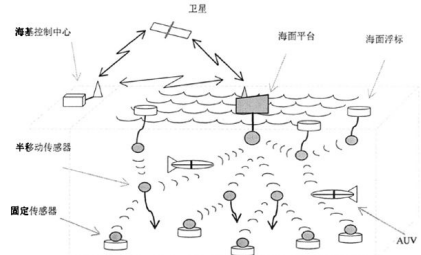
\includegraphics[scale=0.8]{figures/1.png}
	\caption{
		水声传感网络
	}
	\label{fig:example}
\end{figure}

搭载有各种设备的AUV可以在水下按特定轨迹航行,是水下传感网络中常用的移动平台。AUV的加入为海洋立体观测提供了可能,扩大了网络的监控范围;同时AUV可以对网络进行配置,如节点失效时,AUV可以检测通信空洞并指导布放新节点,提高网络的稳健性。
\section{研究内容}
本研究针对有移动节点接入和水下固定传感器组成的小规模单跳网络,结合海洋信息采集中对移动水声传感网络的各类需求,从设计移动节点接入机制、降低整体传输时延等方面入手,进行了如下的研究:
\begin{itemize}
	\item 针对少量移动节点接入固定节点网络,单向采集固定节点数据的场景,设计移动节点的接入和离开机制。移动节点加入固定节点网络时,需要发送广播包通知固定节点进行数据传输,充分利用广播包特点,降低移动节点接入离开机制的开销,是流程设计时的重点。
	\item 当移动节点数量增加时,固定节点传输的目标节点的选择会影响整体网络的性能。在选择目标节点时,一要考虑目标节点与固定节点的远近,这会影响到数据的传输时延;二要考虑目标节点的负载情况,使网络负载相对均衡。因此固定节点要根据实时的网络情况,自适应得进行最优目标节点的选择。
	\item 考虑到水声环境的特殊性,基于RTS/CTS握手机制的竞争协议应用在水声信道中需要进行协议流程和参数的进一步优化。
\end{itemize}

\section{章节安排}
本文的章节安排如下,

第一章绪论,主要介绍了水声传感网络的概念、发展历史和特点,说明了本文的研究背景和应用场景,在此基础上引出了研究的主要内容。

第二章分析了移动水声网络MAC协议研究的国内外现状。

第三章重点介绍了两个竞争型水声传感网络MAC协议,UWALOHA和SFAMA。

第四章针对有移动节点接入的单跳网络,提出了基于竞争的水声UW802.11协议,并详细介绍了协议的流程设计和参数选择。其中,重点介绍了移动节点的接入离开机制和不同网络负载情况下的数据发送机制。

第五章针对提出的UW802.11协议进行理论计算。

第六章介绍了仿真的工具NS2,并且分析了仿真的结果。

\endinput